%
% Section 2: Dataset Results (Insights)
%
%   # of slides: 5 (10-20 new)
%
% -------------------------------------------------------------------------------
\section{Dataset Insights}
\label{sec:data}

\begin{frame}
\frametitle{Datasets and Definitions}

\begin{itemize}

\boxitem{
%
\textcolorbf{colone}{Use 2 CMIP3 GCMs:\;} \ccsm, \hadgem \\[0.5em]
\hspace*{1em} 
last 30 years of climate of the \twentyth century runs (\texttt{20c3m)}.
%
}

\boxitem{ 
%
\textcolorbf{colone}{2 Reanalyses:\;} \era (1969-1999), \ncep (1979-1999).
%
}

\boxitem{\textcolorbf{colone}{Focus on summer:}
%
{
\begin{equation*}
	\text{Summer}\;\equiv\;
	\nicecases{\text{June, July, August}}{if}{\text{NH}}
						{\text{December, January, February}}{\text{SH}}
\end{equation*}
%
}}

\end{itemize}

\end{frame}

\begin{frame}
\frametitle{Temperature Variance Errors}

\begin{center}

\tikzfig{comp_Var_T_bias}{width=\textwidth}

\vspace*{1em}
\tikzitemMark

\end{center}

\begin{tikzpicture}[overlay]

\coordinate (label1) at ($(comp_Var_T_bias.north)+(-3.3,0.1)$);
\coordinate (label2) at ($(comp_Var_T_bias.north)+(2.3,0.1)$);

\node[font={\small \bf}] at (label1) {GCMs};
\node[font={\small \bf}] at (label2) {Reanalyses};

\tikzitem[<1>]{%
%
Plotted as \enskip $\dfrac{\Var(T\subt{dataset})}{\Var(T\subt{observations})}$ 
\enskip,\quad \parbox{0.4\textwidth}{%
%
$T\equiv$ 2-meter temp.\\ 
$T\subt{observations}$ : U. of Delaware
%
}}

\tikzitem[<2>]{%
%
\textcolorbf{coltwo}{Artificial \emph{hot spots} of variability in the GCMs} }

\tikzShadeFig[<2>]{comp_Var_T_bias}{%
  (0.9,0) rectangle (1,1) 
  (0.12, 0.8) circle [radius=0.05]
  (0.25,0.82) circle [radius=0.04]
  (0.12,0.33) circle [radius=0.04]
  (0.26,0.37) circle [radius=0.04]
}

% Reanalyses are not perfect but much better.

\end{tikzpicture}

\end{frame}

\begin{frame}
\frametitle{Summertime mean soil moisture}

\begin{center}

\tikzfig{comp_mbar}{width=0.995\textwidth}

\vspace*{1em}
\tikzitemMark

\end{center}

\begin{tikzpicture}[overlay]

\coordinate (label1) at ($(comp_mbar.north)+(-3.27,0.1)$);
\coordinate (label2) at ($(comp_mbar.north)+(2.34,0.1)$);

\node[font={\small \bf}] at (label1) {GCMs};
\node[font={\small \bf}] at (label2) {Reanalyses};

\tikzitem[<1>]{\parbox{0.8\textwidth}{\centering%
%
Soil moisture content in the top 10$\cm$ of soil:\, $\mbar$ \\[1ex]
Saturation $\simeq$ 65 $\mm$}}

\tikzitem[<2>]{%
%
\textcolorbf{coltwo}{GCMs are overall \emph{much} dryer} }

\tikzShadeFig[<2>]{comp_mbar}{%
  (0.9,0) rectangle (1,1) 
  (0.12,0.8) circle [radius=0.05]
  (0.25,0.82) circle [radius=0.04]
  (0.12,0.33) circle [radius=0.04]
  (0.26,0.37) circle [radius=0.04]
  (0.56,0.8) circle [radius=0.05]
  (0.69,0.82) circle [radius=0.04]
  (0.56,0.33) circle [radius=0.04]
  (0.69,0.37) circle [radius=0.04]
}

%%

\end{tikzpicture}

\end{frame}

\begin{frame}
\frametitle{Correlations {\normalsize involving Evapotranspiration\; (1/2)}}

\begin{columns}

\begin{column}{0.4\linewidth}

\vspace*{-1em}

\begin{itemize}

%\boxitem[0.80][<1->]{\textcolorbf{colone}{\centering
%A clear\\ dichotomy pattern} } 
%
%\vspace*{-0.5em}

\boxitem[0.80][<2->]{\textcolorbf{colone}{\centering
%
How can $E$ decrease \\ 
when $F$ , $m$ \\ \hspace*{1.8em} increase ?} }

\vspace*{-0.9em}

\boxitem[0.80][<3->]{\centering%
%
 \textcolorbf{coltwo}{Dry soils} \\[-0.5ex]
{\small ($\mbar<$  global mean)} \\[-0.4ex]
 \textcolorbf{coltwo}{$\iff$} \\[-0.4ex]
 \textcolorbf{coltwo}{Moisture-limited} \\[-0.5ex]
{\small ($\corr(E,m)>0$)} \\[1em]
% 
\uncover<4->{%
%
 \textcolorbf{coltwo}{Wet soils} \\[-0.5ex]
{\small ($\mbar>$  global mean)} \\[-0.4ex]
 \textcolorbf{coltwo}{$\iff$} \\[-0.4ex]
 \textcolorbf{coltwo}{Energy-limited} \\[-0.5ex]
{\small ($\corr(E,F)>0$)} }
%
}

\end{itemize}

\end{column}

\begin{column}{0.6\linewidth}

\uncover<1-2>{%
%
\vspace*{1.5em}
\tikzfig{hadgem1_Cor_EF_Cor_Em}{width=\linewidth} }

\end{column}

\end{columns}

\begin{tikzpicture}[overlay]

% title and data
\coordinate (title) at ($(hadgem1_Cor_EF_Cor_Em.north)+(-0.4,0.6)$);
\node[color=colone,font=\bf] at (title) {$E\;\,$ with $F$ , $m$};
\coordinate (data) at ($(hadgem1_Cor_EF_Cor_Em.south)+(-0.4,-0.3)$);
\node[color=colone,font=\bf] at (data) {[\hadgem data]};

% pt 1 
\definecolor{p-1}{RGB}{255,255,51}  % yellow
\coordinate (p-1) at ($(hadgem1_Cor_EF_Cor_Em.west)+(1.5,1.7)$);
\coordinate (p-11) at ($(hadgem1_Cor_EF_Cor_Em.west)+(1.5,-1.1)$);
\uncover<2->{%
%
\node[color=p-1,scale=1.5] at (p-1) {\textbullet};
\node[color=p-1,scale=1.5] at (p-11) {\textbullet}; }

% pt 2
%\definecolor{p-2}{RGB}{252,141,98} % orange
\coordinate (p-2) at ($(hadgem1_Cor_EF_Cor_Em.west)+(2.3,0.8)$);
\coordinate (p-22) at ($(hadgem1_Cor_EF_Cor_Em.west)+(2.3,-2)$);
\uncover<2->{%
%
\node[color=p-1,scale=1.5] at (p-2) {\textbullet};
\node[color=p-1,scale=1.5] at (p-22) {\textbullet}; }

% superposed figure (same width as column) + dry soils pt
\coordinate (superposed) at ($(hadgem1_Cor_EF_Cor_Em.north)+(-0.4,0.1)$);
\uncover<3->{%
%
\node at (hadgem1_Cor_EF_Cor_Em) 
  {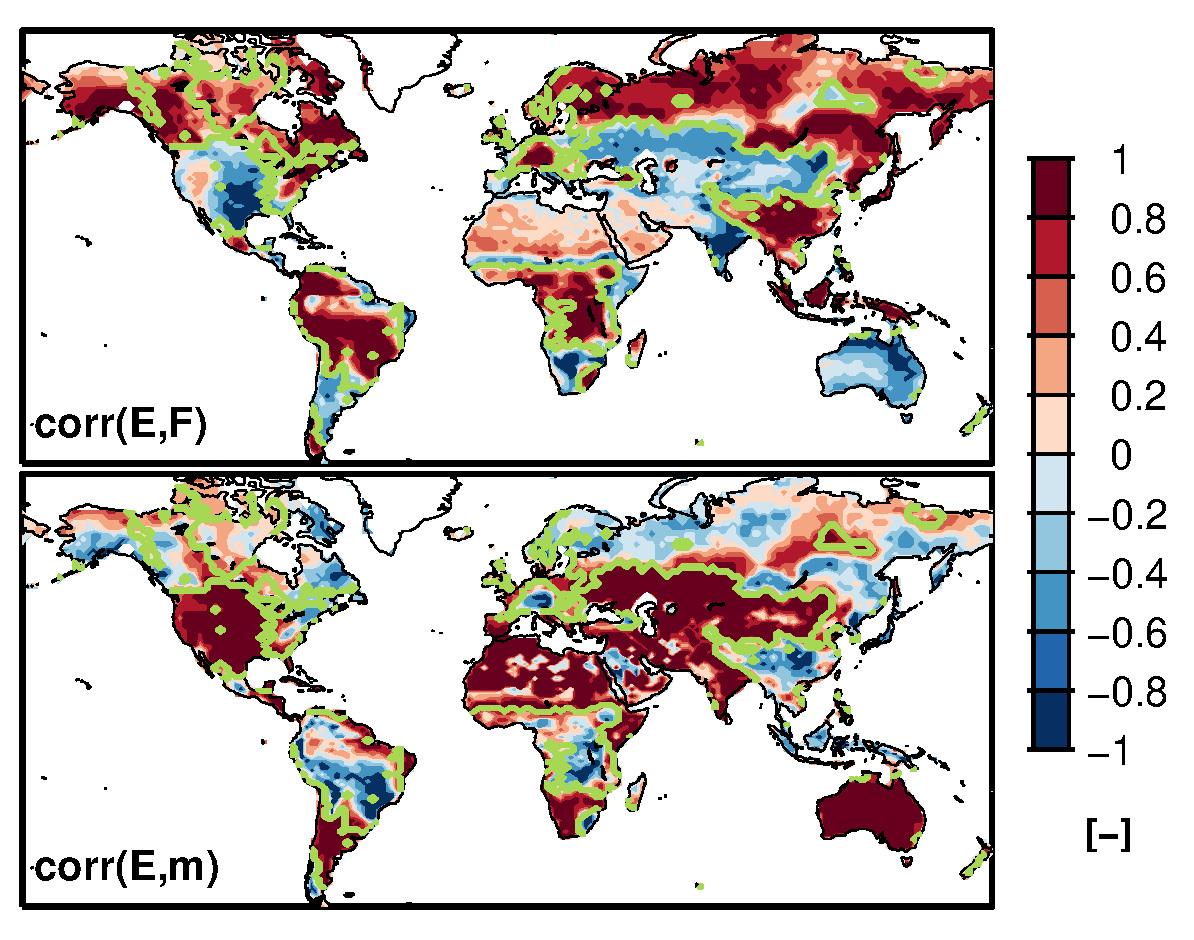
\includegraphics[width=0.6\linewidth]{hadgem1_Cor_EF_Cor_Em_OvGM}}; 
\node[color=colone,font=\bf] at (superposed) 
  {$\mbar\;=\;$ global mean value};
\node[color=p-1,scale=1.5] at (p-1) {\textbullet};
\node[color=p-1,scale=1.5] at (p-11) {\textbullet}; }

% wet point pt
\uncover<4->{%
%
\node[color=p-1,scale=1.5] at (p-2) {\textbullet};
\node[color=p-1,scale=1.5] at (p-22) {\textbullet};  }

\end{tikzpicture}

\end{frame}

\begin{frame}
\frametitle{Correlations {\normalsize involving Evapotranspiration\; (2/2)}}

\begin{columns}

\begin{column}{0.45\linewidth}

\vspace*{-2em}

\begin{itemize}

\item<1-> Decompose radiation forcing anomalies into \\ 
\textcolorbf{colone}{non-precipitating} and \\ 
\textcolorbf{colone}{precipitating} components:

\begin{equation}
  F' \;=\; F_0' \;-\; L\alpha\,  P'
\end{equation}

where $\innerp{F_0'}{P'}\equiv0$, \\ 
$\alpha>0$ (unitless)

%\item<3-> \textcolorbf{colone}{superpose the line where \\ 
%$\mbar$ is equal to the \\ 
%global mean value}

\boxitem[0.82][<3->]{%
%
\textcolorbf{coltwo}{Over dry soils: $F'{>}0$ \\ 
\hspace*{1ex} $\iff$ moisture deficit} \\[0.5em]
%
\textcolorbf{coltwo}{Over wet soils: $m'{>}0$ \\
\hspace*{1ex} $\iff$ energy deficit} }

\end{itemize}

\end{column}

\hfill

\begin{column}{0.52\linewidth}

\vspace*{-0.5em}
\tikzfig{hadgem1_Cor_EF_Cor_Em_Cor_EF0_OvGM}{width=\linewidth}

\end{column}

\end{columns}

\begin{tikzpicture}[overlay]

\coordinate (data) at ($(hadgem1_Cor_EF_Cor_Em_Cor_EF0_OvGM.south)+(-0.4,-0.25)$);

\node[color=colone,font=\bf] at (data) {[\hadgem data]};

\tikzCoverFig[<1>]{hadgem1_Cor_EF_Cor_Em_Cor_EF0_OvGM}{%
  (0,0) rectangle (0.83,0.34)
}

\definecolor{p-1}{RGB}{255,255,51}  % yellow
\coordinate (p-1) at ($(hadgem1_Cor_EF_Cor_Em_Cor_EF0_OvGM.west)+(1.35,2.7)$);
\coordinate (p-11) at ($(hadgem1_Cor_EF_Cor_Em_Cor_EF0_OvGM.west)+(1.35,0.3)$);
\coordinate (p-111) at ($(hadgem1_Cor_EF_Cor_Em_Cor_EF0_OvGM.west)+(1.35,-2.15)$);
\uncover<2>{%
%
\node[color=p-1,scale=1.5] at (p-1) {\textbullet};
\node[color=p-1,scale=1.5] at (p-11) {\textbullet};
\node[color=p-1,scale=1.5] at (p-111) {\textbullet}; }

\end{tikzpicture}

\end{frame}

% -------------------------------------------------------------------------------
